\section{Optimal Communication Chain over the Ideal Channel}
\subsection{Communication Chain}
\begin{figure}[H]
	\centering
	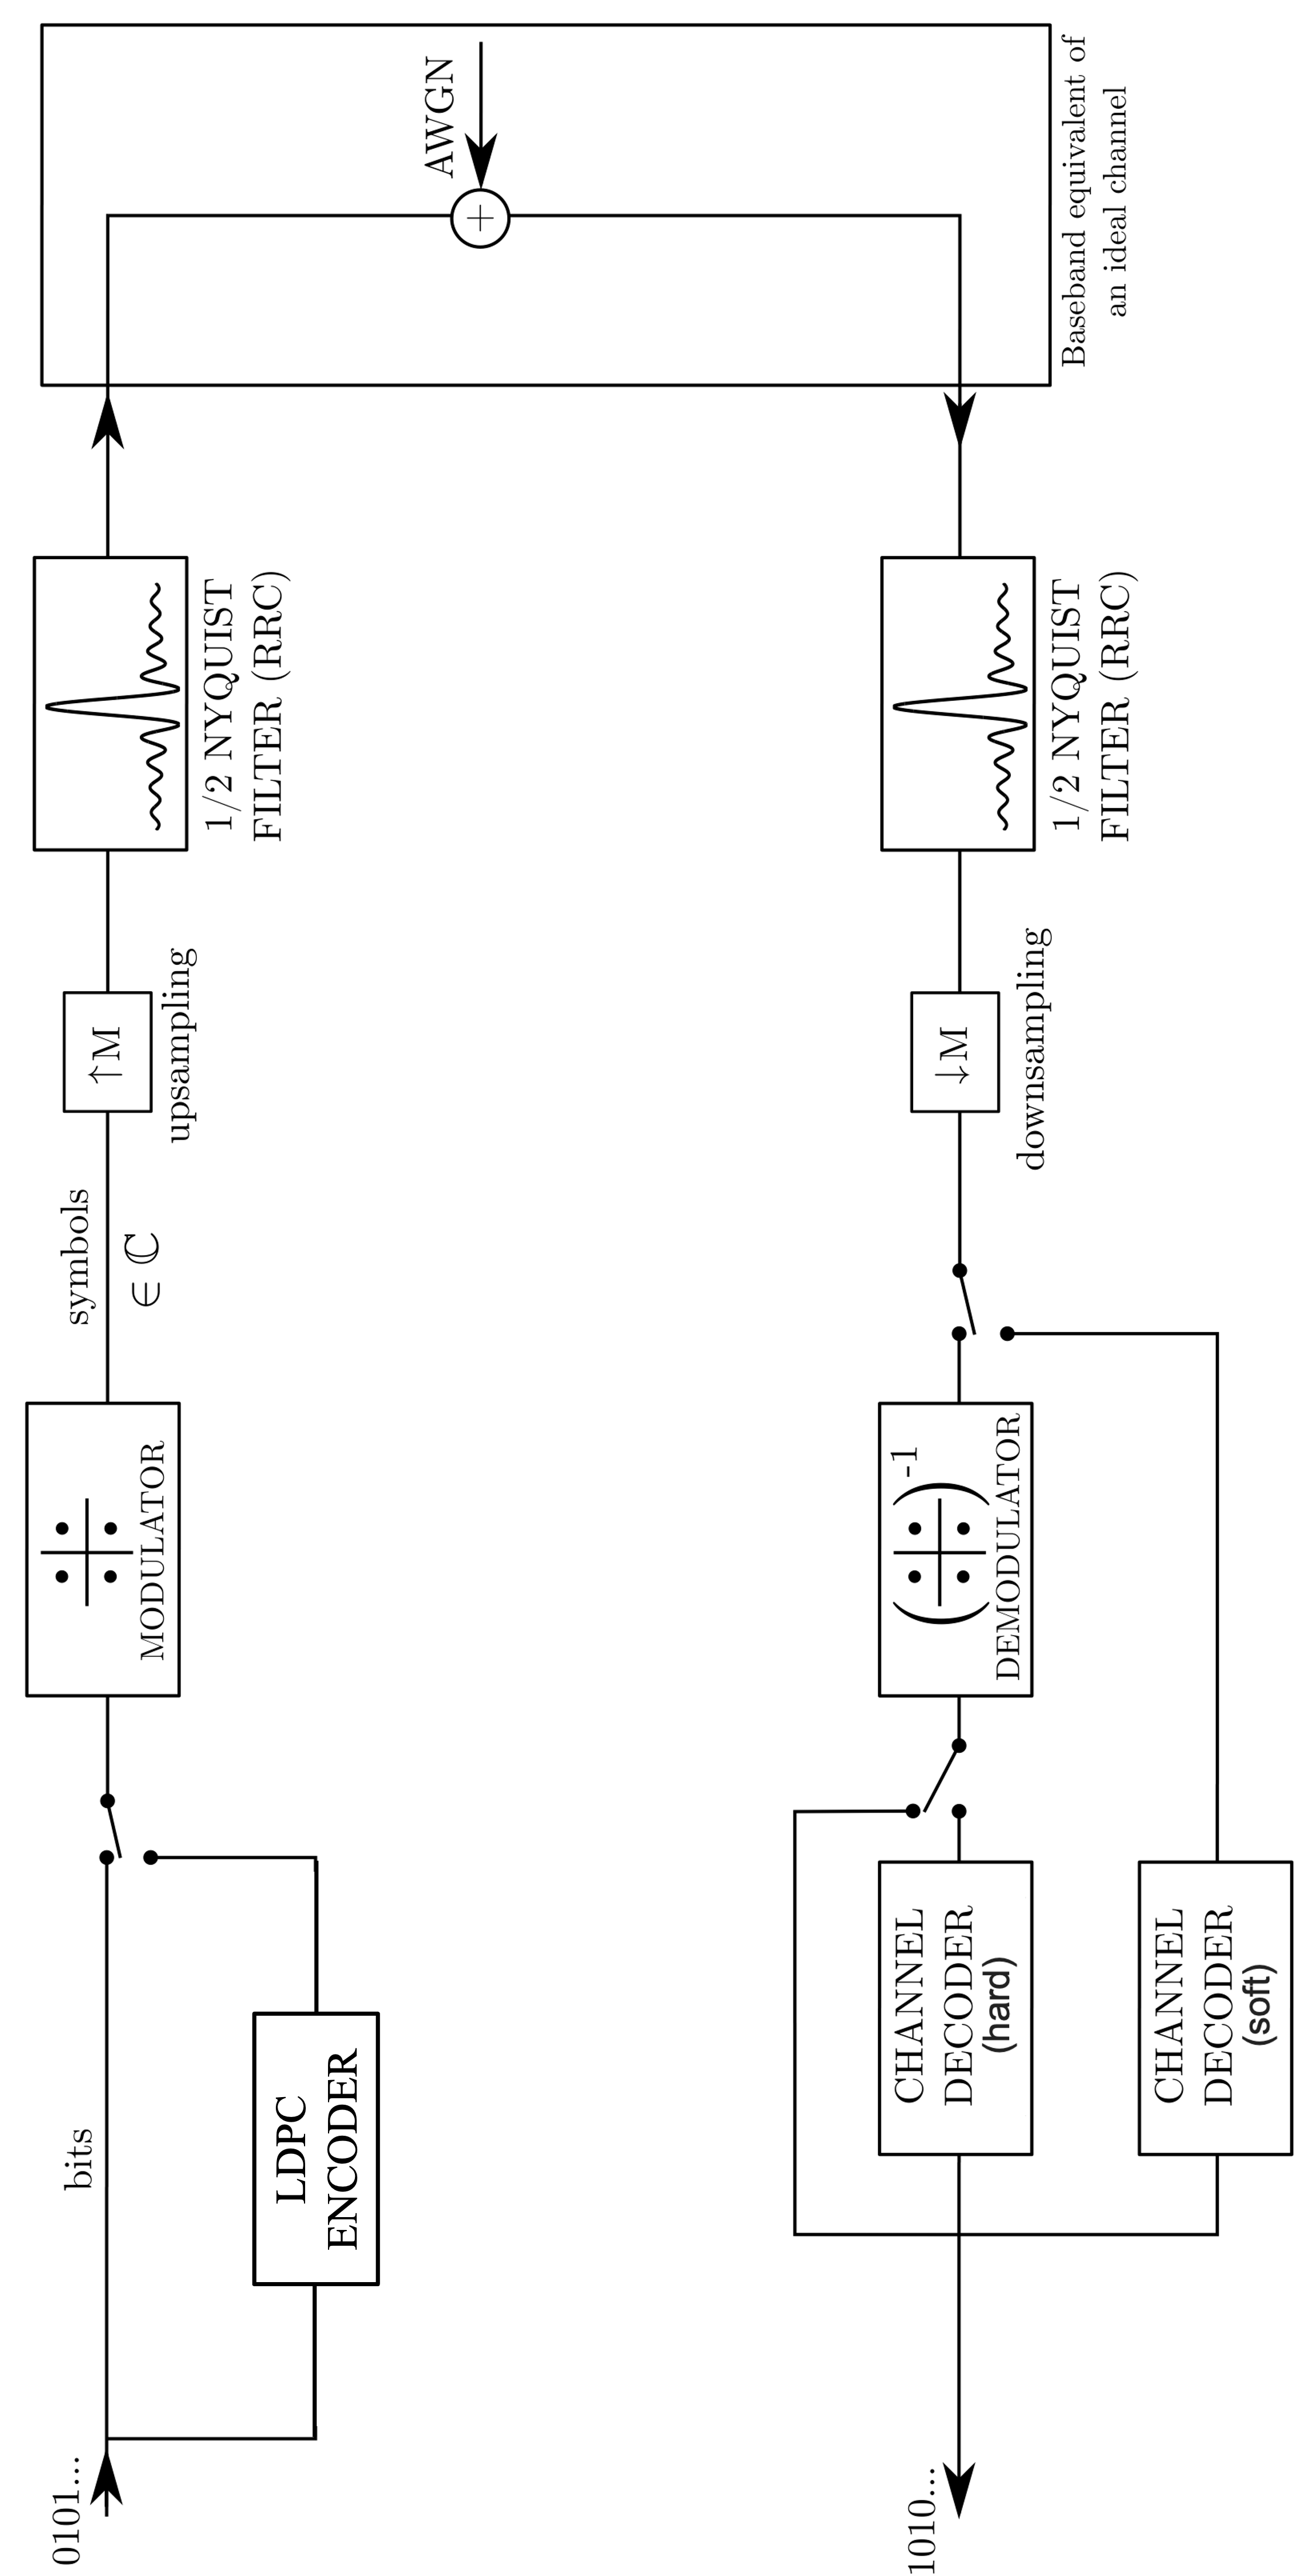
\includegraphics[angle=-90, width=0.9\linewidth]{Images/com-chain}
	\caption{Block diagram of the communication system}
	\label{fig:com-chain}
\end{figure}
The communication chain depicted in Figure \ref{fig:com-chain} models the pipeline of a DVB-C transmitter and receiver at baseband. On the transmitter side, there is a generation of a bit-stream, which is then mapped to complex symbols from a chosen QAM modulation. These symbols are subsequently up-sampled and shaped by a half-root Nyquist filter to limit their bandwidth. On the receiver's side, the signal transmitted is matched-filtered with the same half-root Nyquist filter. The goal of this matched filter is to maximize the signal-to-noise ratio. The output of the matched filter is then down-sampled at the symbols instances, and then demapped to recover an estimate of the bit-stream transmitted.\\
In this project, the Low Density Parity Check Encoder is not implemented, and the algorithm for symbols mapping and demapping were provided.



\subsection{Bit Generation and Symbol Mapping and Demapping}
Symbols mapping is the process in which the modulator transforms a sequence of bits into a sequence of complex symbols. This helps improving the spectral efficiency as it allows more bits to be transmitted per symbol over a given bandwidth.\\
At the receiver end, symbol demapping is performed to convert noisy symbols back into an estimated sequence of bits. This is done through Maximum Likelihood criterion, which aims to selecting the constellation symbol that is closest to the received sample in minimum Euclidean distance.

\begin{equation}
	\tilde{\underline{s}}_{m}^{ML} = \max_{\underline{s}_{m}} (\ln p(\underline{r}|\underline{s}_{m})) = \min_{\underline{s}_{m}} \left(\sum_{k=1}^{K}(r_{k}-s_{mk})^{2}\right)
\end{equation}

Where:
\begin{itemize}
	\item $\tilde{\underline{s}}_{m}^{ML}$ is the estimated symbol using the Maximum Likelihood criterion.
	\item $\underline{r} = [r_1, r_2, \dots, r_K]^T$ is the received vector after demodulation 
	\item $\underline{s}_{m} = [s_{m1}, s_{m2}, \dots, s_{mK}]^T$ is the vector representing the $m$-th possible transmitted symbol.
	\item $p(\underline{r}|\underline{s}_{m})$ is the conditional probability of receiving vector $\underline{r}$ given that symbol $\underline{s}_m$ was sent.
	\item $\sum_{k=1}^{K}(r_{k}-s_{mk})^{2}$ represents the squared Euclidean distance between the received vector $\underline{r}$ and the symbol vector $\underline{s}_m$.
\end{itemize}

\subsection{Nyquist Filtering}
After mapping the bit-stream into symbols, the sequence of complex symbols $I[n]$ is up-sampled by a factor of $M > 1$, before passing through a pulse shaping filter $g(t)$. The purpose of this filtering is to
\begin{enumerate}
	\item To limit the bandwidth of the transmitted signal
	\item To control the interference between successive symbols
\end{enumerate}
\subsubsection{Half-Root Nyquist Filter Design and Matched Filtering}
To achieve optimal performance in terms of ISI cancellation and maximizing the SNR at the receiver, a root-raised cosine filter is used. This filter ensures that the overall desired channel response $h(t)$, from the input symbols at the transmitter to the sampled symbols at the receiver, satisfies the Nyquist criterion for zero ISI. This criterion states that the normalized impulse response of the equivalent discrete-time channel $h(nT_{symb})$  is such that
\begin{equation}
	h(nT_{symb}) = \begin{cases}
		1 & n=0 \\
		0 & n \neq 0
	\end{cases}
\end{equation}

The filtering is split between a root-raised cosine (RRC) pulse shaping filter $g(t)$ at the transmitter and its matched version $g^*(-t)$ at the receiver. The convolution in the time domain of these two filters, $h(t) = g(t) \otimes g^*(-t)$, forms the overall channel response that satisfies the Nyquist criterion for zero ISI.
To design the root-raised cosine filter $g(t)$, the transfer function of the raised cosine filter $H(f)$ is first defined. A square root is then performed on $H(f)$ to find the frequency response of the RRC filter, $G(f) = \sqrt{H(f)}$. Afterwards, an inverse Fourier transform is computed to find its time-domain equivalent $g(t)$.\\

The frequency response of the raised cosine filter $H(f)$ is equivalent to a rectangular window, but with a slope that is less sharp and characterized by a roll-off factor $\beta = 0.2$. Thus its frequency response is given by:

\begin{equation}
	H(f) = \begin{cases}
		T_{symb} & 0 \le |f| < \frac{1-\beta}{2T} \\
		\frac{T_{symb}}{2} \left(1 + \cos\left[\frac{\pi T_{symb}}{\beta}\left(|f| - \frac{1-\beta}{2T}\right)\right]\right) & \frac{1-\beta}{2T} \le |f| \le \frac{1+\beta}{2T} \\
		0 & |f| > \frac{1+\beta}{2T}
	\end{cases}
\end{equation}

When the time domain impulse response of the raised-cosine filter is sampled at the symbol rate, it is equivalent to a dirac pulse.



\subsubsection{Filter Properties and Inter Symbol Interference Cancellation}
\subsection{Noise Addition and Performance Evaluation}
\subsection{Questions and Answers}